\documentclass{beamer}
\usetheme{default}

\title{SAT solvers and Applications to Combinatorics }
\date{}
\usepackage{amsmath}
\usepackage{amsfonts} % Fonts like \mathbb and \mathcal
\usepackage{amssymb}
\newcommand{\divides}{\mid}
\newcommand{\notdivides}{\nmid}

\usepackage{listings}
\newcommand{\Z}{\mathbb{Z}}
\newcommand{\N}{\mathbb{N}}
\newcommand{\BigO}{\mathcal{O}}
\newcommand{\parenmod}[1]{(\text{mod } #1)}
\usepackage{hyperref}

%slide 1
\begin{document}
\begin{frame}[plain]
    \maketitle
\end{frame}

%slide 2
\begin{frame}{Introduction - Boolean formulas}
	\begin{itemize}
		\item A Boolean formula is an expression involving Boolean variables and the three operations $\wedge$ 'and', $\vee$ 'or' and  $\neg$ for negation.
		$$\phi = (x\vee y) \wedge (z \vee \neg y)$$
		\item \textbf{Definition:} A Boolean formula is \textit{satisfiable} if and only if there exist at least one variable assignment to the variables to the formula which evaluates it to True. 
		\item $\phi$ is satisfiable with assignment $x$ is true, $y$ is false $z$ is true. 
	\end{itemize}
\end{frame}

%slide 3
\begin{frame}{SAT and CNF Encodings}

	\begin{itemize}
		\item The Boolean Satisfiability problem(SAT) is to test whether a given Boolean formula is satisfiable.
		\item In order to uniform the formatting of SAT problems and for the easy of storing, usually the Boolean formula is transformed into conjunctive normal form(CNF).
		\item CNF is a conjunction of clauses $\bigwedge_{i} c_i$, each clause $c_i$ being a disjunction of literals $\bigvee_i l_i$ and each literal $l_i$ being either a Boolean variable $v$ or its negation $\neg v$. 
	\end{itemize}
\end{frame}

%small digression
\begin{frame}{SAT solver}

	\begin{itemize}
		\item There are many SAT solvers out there, with varying efficiency. The state-of-the-art solvers include Satch and MiniSat and others. 
		\item Most of the SAT solvers is based in the Davis-Putnam-Logemann-Loveland(DPLL) algorithm.
		\item Satch in action
		\item DPLL algorithm high-level example
	\end{itemize}
\end{frame}


%slide 4
\begin{frame}[t]{Combinatorics Example}

	\begin{itemize}
		\item \textbf{Definition:} MinColoring problem states that, given a graph $G$, find the minimum number of colors which G's vertices can be colored.  
		\item Given a graph $G = (V,E)$ and an integer $k$, is the graph k-colorable? 
		\item Encode the vertex coloring: 
		$$\phi_v = \bigwedge_{v_i \in V} (v_{i}^1 \vee v_{i}^2 \vee \dots v_{i}^k) \wedge \neg (v_{i}^1 \wedge v_{i}^2 \wedge \dots v_{i}^k)$$
		\item Encode the edges: 
		$$\phi_E = \bigwedge_{(v_i, v_j) \in E} (\neg (v_{i}^1 \wedge v_{j}^1) \wedge \neg (v_{i}^2 \wedge v_{j}^2) \wedge \dots \neg (v_{i}^k \wedge v_{j}^k))$$
		\item The resulting formula for SAT solver is 
		$$\psi = \phi_v \wedge \phi_E$$
	\end{itemize}

\end{frame}

%slide CNF encoding
\begin{frame}{CNF file format}
	\begin{itemize}
		\item In order for a SAT solver to take in the input, the CNF form also must be formatted in a particular way. 
		\item The CNF file needs to have a parameter line starting with 'p', followed with 'cnf' indicating its cnf form. Next, followed with 2 numbers representing the number of literals and clauses respectively. 
		\item Following the parameter line are the clauses.
		\item Each clause(line) must end with a '0'.
		\item Variables must be non-zero numbers, negated literals will have a minus sign. 
		\item Comments start with a 'c' in the beginning. 
		\item File must end with a newline character.
	\end{itemize}

\end{frame}

%slide CNF file example
% is a simple square 2-colorable?
\begin{frame}{CNF file example}

	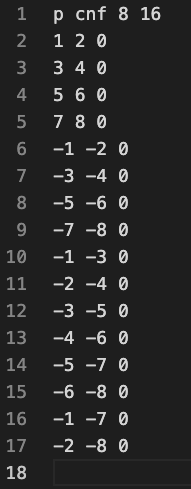
\includegraphics[scale=0.4]{cnf_example}

\end{frame}


\begin{frame}[t]{DPLL}

	\begin{itemize}
		\item Within the SAT solver, what is the algorithm?
		\item DPLL consists of 3 main actions.
		\begin{itemize}
			\item Decision - randomly assign a literal true or false
			\item Unit propagation - must assign a unit literal with a value
			\item Backtracking - backtracking to a previous decision at conflicts(contradiction)
		\end{itemize}
		\item A unit clause is a clause where a single literal in it is unassigned and the rest are false. That unassigned literal is called unit literal.
		\item The algorithm executes in the order of: check for backtracking $\to$ check the need for unit propagation $\to$ make a decision.
		\item Let's see a quick example to solidify understanding. 
	\end{itemize}

\end{frame}

\begin{frame}[t]{DPLL example}
	$(x_1 \vee x_2)$ \\
	$(x_1 \vee x_2 \vee x_8)$\\
	$(\neg x_2 \vee \neg x_3 \vee x_4)$\\
	$(\neg x_4 \vee x_5 \vee x_7)$\\
	$(\neg x_4 \vee x_6 \vee x_8)$\\
	$(\neg x_5 \vee \neg x_6)$\\
	$(x_7 \vee \neg x_8)$\\
	$(x_7 \vee x_9 \vee x_{10})$\\
	\bigbreak
	\begin{itemize}
		\item Begin with unit propagation.
		\item Randomly make a decision, $x_7 = 0$?
	\end{itemize}
	
\end{frame}


\begin{frame}{DPLL Optimization}
	\begin{itemize}
		\item The number of clauses grows very fast. For $K_6$, there are ${6 \choose 2} = 15$ edges. Thus, $2^{15} = 32,768$ different way of coloring the graph.
		\item Optimization for DPLL, \textbf{clause learning}.
		\item Quicker unit propagation with Two-Watch-Literal invariant.
		\item Weighted decision instead of random.
		\item Parallelize the problem with clever encoding.
		\item Parallel Multithreaded SAT solver.
	
	\end{itemize}
\end{frame}

\begin{frame}{Application to Ramsey Number}
	
	\begin{itemize}
		\item The area that Jack and I will be focusing on is Ramsey Numbers.
		\item Using efficient implementation of SAT solvers to potentially improve the bounds on some Ramsey numbers. 
	\end{itemize}
    
\end{frame}

\end{document}






















